% Options for packages loaded elsewhere
\PassOptionsToPackage{unicode}{hyperref}
\PassOptionsToPackage{hyphens}{url}
%
\documentclass[
  man]{apa6}
\usepackage{amsmath,amssymb}
\usepackage{iftex}
\ifPDFTeX
  \usepackage[T1]{fontenc}
  \usepackage[utf8]{inputenc}
  \usepackage{textcomp} % provide euro and other symbols
\else % if luatex or xetex
  \usepackage{unicode-math} % this also loads fontspec
  \defaultfontfeatures{Scale=MatchLowercase}
  \defaultfontfeatures[\rmfamily]{Ligatures=TeX,Scale=1}
\fi
\usepackage{lmodern}
\ifPDFTeX\else
  % xetex/luatex font selection
\fi
% Use upquote if available, for straight quotes in verbatim environments
\IfFileExists{upquote.sty}{\usepackage{upquote}}{}
\IfFileExists{microtype.sty}{% use microtype if available
  \usepackage[]{microtype}
  \UseMicrotypeSet[protrusion]{basicmath} % disable protrusion for tt fonts
}{}
\makeatletter
\@ifundefined{KOMAClassName}{% if non-KOMA class
  \IfFileExists{parskip.sty}{%
    \usepackage{parskip}
  }{% else
    \setlength{\parindent}{0pt}
    \setlength{\parskip}{6pt plus 2pt minus 1pt}}
}{% if KOMA class
  \KOMAoptions{parskip=half}}
\makeatother
\usepackage{xcolor}
\usepackage{graphicx}
\makeatletter
\def\maxwidth{\ifdim\Gin@nat@width>\linewidth\linewidth\else\Gin@nat@width\fi}
\def\maxheight{\ifdim\Gin@nat@height>\textheight\textheight\else\Gin@nat@height\fi}
\makeatother
% Scale images if necessary, so that they will not overflow the page
% margins by default, and it is still possible to overwrite the defaults
% using explicit options in \includegraphics[width, height, ...]{}
\setkeys{Gin}{width=\maxwidth,height=\maxheight,keepaspectratio}
% Set default figure placement to htbp
\makeatletter
\def\fps@figure{htbp}
\makeatother
\setlength{\emergencystretch}{3em} % prevent overfull lines
\providecommand{\tightlist}{%
  \setlength{\itemsep}{0pt}\setlength{\parskip}{0pt}}
\setcounter{secnumdepth}{-\maxdimen} % remove section numbering
% Make \paragraph and \subparagraph free-standing
\makeatletter
\ifx\paragraph\undefined\else
  \let\oldparagraph\paragraph
  \renewcommand{\paragraph}{
    \@ifstar
      \xxxParagraphStar
      \xxxParagraphNoStar
  }
  \newcommand{\xxxParagraphStar}[1]{\oldparagraph*{#1}\mbox{}}
  \newcommand{\xxxParagraphNoStar}[1]{\oldparagraph{#1}\mbox{}}
\fi
\ifx\subparagraph\undefined\else
  \let\oldsubparagraph\subparagraph
  \renewcommand{\subparagraph}{
    \@ifstar
      \xxxSubParagraphStar
      \xxxSubParagraphNoStar
  }
  \newcommand{\xxxSubParagraphStar}[1]{\oldsubparagraph*{#1}\mbox{}}
  \newcommand{\xxxSubParagraphNoStar}[1]{\oldsubparagraph{#1}\mbox{}}
\fi
\makeatother
% definitions for citeproc citations
\NewDocumentCommand\citeproctext{}{}
\NewDocumentCommand\citeproc{mm}{%
  \begingroup\def\citeproctext{#2}\cite{#1}\endgroup}
\makeatletter
 % allow citations to break across lines
 \let\@cite@ofmt\@firstofone
 % avoid brackets around text for \cite:
 \def\@biblabel#1{}
 \def\@cite#1#2{{#1\if@tempswa , #2\fi}}
\makeatother
\newlength{\cslhangindent}
\setlength{\cslhangindent}{1.5em}
\newlength{\csllabelwidth}
\setlength{\csllabelwidth}{3em}
\newenvironment{CSLReferences}[2] % #1 hanging-indent, #2 entry-spacing
 {\begin{list}{}{%
  \setlength{\itemindent}{0pt}
  \setlength{\leftmargin}{0pt}
  \setlength{\parsep}{0pt}
  % turn on hanging indent if param 1 is 1
  \ifodd #1
   \setlength{\leftmargin}{\cslhangindent}
   \setlength{\itemindent}{-1\cslhangindent}
  \fi
  % set entry spacing
  \setlength{\itemsep}{#2\baselineskip}}}
 {\end{list}}
\usepackage{calc}
\newcommand{\CSLBlock}[1]{\hfill\break\parbox[t]{\linewidth}{\strut\ignorespaces#1\strut}}
\newcommand{\CSLLeftMargin}[1]{\parbox[t]{\csllabelwidth}{\strut#1\strut}}
\newcommand{\CSLRightInline}[1]{\parbox[t]{\linewidth - \csllabelwidth}{\strut#1\strut}}
\newcommand{\CSLIndent}[1]{\hspace{\cslhangindent}#1}
\ifLuaTeX
\usepackage[bidi=basic]{babel}
\else
\usepackage[bidi=default]{babel}
\fi
\babelprovide[main,import]{english}
% get rid of language-specific shorthands (see #6817):
\let\LanguageShortHands\languageshorthands
\def\languageshorthands#1{}
% Manuscript styling
\usepackage{upgreek}
\captionsetup{font=singlespacing,justification=justified}

% Table formatting
\usepackage{longtable}
\usepackage{lscape}
% \usepackage[counterclockwise]{rotating}   % Landscape page setup for large tables
\usepackage{multirow}		% Table styling
\usepackage{tabularx}		% Control Column width
\usepackage[flushleft]{threeparttable}	% Allows for three part tables with a specified notes section
\usepackage{threeparttablex}            % Lets threeparttable work with longtable

% Create new environments so endfloat can handle them
% \newenvironment{ltable}
%   {\begin{landscape}\centering\begin{threeparttable}}
%   {\end{threeparttable}\end{landscape}}
\newenvironment{lltable}{\begin{landscape}\centering\begin{ThreePartTable}}{\end{ThreePartTable}\end{landscape}}

% Enables adjusting longtable caption width to table width
% Solution found at http://golatex.de/longtable-mit-caption-so-breit-wie-die-tabelle-t15767.html
\makeatletter
\newcommand\LastLTentrywidth{1em}
\newlength\longtablewidth
\setlength{\longtablewidth}{1in}
\newcommand{\getlongtablewidth}{\begingroup \ifcsname LT@\roman{LT@tables}\endcsname \global\longtablewidth=0pt \renewcommand{\LT@entry}[2]{\global\advance\longtablewidth by ##2\relax\gdef\LastLTentrywidth{##2}}\@nameuse{LT@\roman{LT@tables}} \fi \endgroup}

% \setlength{\parindent}{0.5in}
% \setlength{\parskip}{0pt plus 0pt minus 0pt}

% Overwrite redefinition of paragraph and subparagraph by the default LaTeX template
% See https://github.com/crsh/papaja/issues/292
\makeatletter
\renewcommand{\paragraph}{\@startsection{paragraph}{4}{\parindent}%
  {0\baselineskip \@plus 0.2ex \@minus 0.2ex}%
  {-1em}%
  {\normalfont\normalsize\bfseries\itshape\typesectitle}}

\renewcommand{\subparagraph}[1]{\@startsection{subparagraph}{5}{1em}%
  {0\baselineskip \@plus 0.2ex \@minus 0.2ex}%
  {-\z@\relax}%
  {\normalfont\normalsize\itshape\hspace{\parindent}{#1}\textit{\addperi}}{\relax}}
\makeatother

\makeatletter
\usepackage{etoolbox}
\patchcmd{\maketitle}
  {\section{\normalfont\normalsize\abstractname}}
  {\section*{\normalfont\normalsize\abstractname}}
  {}{\typeout{Failed to patch abstract.}}
\patchcmd{\maketitle}
  {\section{\protect\normalfont{\@title}}}
  {\section*{\protect\normalfont{\@title}}}
  {}{\typeout{Failed to patch title.}}
\makeatother

\usepackage{xpatch}
\makeatletter
\xapptocmd\appendix
  {\xapptocmd\section
    {\addcontentsline{toc}{section}{\appendixname\ifoneappendix\else~\theappendix\fi: #1}}
    {}{\InnerPatchFailed}%
  }
{}{\PatchFailed}
\makeatother
\keywords{keywords\newline\indent Word count: X}
\DeclareDelayedFloatFlavor{ThreePartTable}{table}
\DeclareDelayedFloatFlavor{lltable}{table}
\DeclareDelayedFloatFlavor*{longtable}{table}
\makeatletter
\renewcommand{\efloat@iwrite}[1]{\immediate\expandafter\protected@write\csname efloat@post#1\endcsname{}}
\makeatother
\usepackage{lineno}

\linenumbers
\usepackage{csquotes}
\ifLuaTeX
  \usepackage{selnolig}  % disable illegal ligatures
\fi
\usepackage{bookmark}
\IfFileExists{xurl.sty}{\usepackage{xurl}}{} % add URL line breaks if available
\urlstyle{same}
\hypersetup{
  pdftitle={Data Exercise 3},
  pdfauthor={First Author1 \& Ernst-August Doelle1,2},
  pdflang={en-EN},
  pdfkeywords={keywords},
  hidelinks,
  pdfcreator={LaTeX via pandoc}}

\title{Data Exercise 3}
\author{First Author\textsuperscript{1} \& Ernst-August Doelle\textsuperscript{1,2}}
\date{}


\shorttitle{Title}

\authornote{

Add complete departmental affiliations for each author here. Each new line herein must be indented, like this line.

Enter author note here.

The authors made the following contributions. First Author: Conceptualization, Writing - Original Draft Preparation, Writing - Review \& Editing; Ernst-August Doelle: Writing - Review \& Editing, Supervision.

Correspondence concerning this article should be addressed to First Author, Postal address. E-mail: \href{mailto:my@email.com}{\nolinkurl{my@email.com}}

}

\affiliation{\vspace{0.5cm}\textsuperscript{1} Wilhelm-Wundt-University\\\textsuperscript{2} Konstanz Business School}

\abstract{%
One or two sentences providing a \textbf{basic introduction} to the field, comprehensible to a scientist in any discipline.
Two to three sentences of \textbf{more detailed background}, comprehensible to scientists in related disciplines.
One sentence clearly stating the \textbf{general problem} being addressed by this particular study.
One sentence summarizing the main result (with the words ``\textbf{here we show}'' or their equivalent).
Two or three sentences explaining what the \textbf{main result} reveals in direct comparison to what was thought to be the case previously, or how the main result adds to previous knowledge.
One or two sentences to put the results into a more \textbf{general context}.
Two or three sentences to provide a \textbf{broader perspective}, readily comprehensible to a scientist in any discipline.
}



\begin{document}
\maketitle

\subsection{Themes}\label{themes}

\section{Methods}\label{methods}

We report how we determined our sample size, all data exclusions (if any), all manipulations, and all measures in the study.

\subsection{Participants}\label{participants}

\subsection{Material}\label{material}

\subsection{Procedure}\label{procedure}

\subsection{Data analysis}\label{data-analysis}

We used R (Version 4.4.1; R Core Team, 2024) and the R-packages \emph{dplyr} (Version 1.1.4; Wickham, François, Henry, Müller, \& Vaughan, 2023), \emph{forcats} (Version 1.0.0; Wickham, 2023a), \emph{ggdist} (Version 3.3.2; Kay, 2024), \emph{ggplot2} (Version 3.5.1; Wickham, 2016), \emph{lubridate} (Version 1.9.3; Grolemund \& Wickham, 2011), \emph{papaja} (Version 0.1.3; Aust \& Barth, 2024), \emph{purrr} (Version 1.0.2; Wickham \& Henry, 2023), \emph{readr} (Version 2.1.5; Wickham, Hester, \& Bryan, 2024), \emph{stringr} (Version 1.5.1; Wickham, 2023b), \emph{tibble} (Version 3.2.1; Müller \& Wickham, 2023), \emph{tidyr} (Version 1.3.1; Wickham, Vaughan, \& Girlich, 2024), \emph{tidyverse} (Version 2.0.0; Wickham et al., 2019) and \emph{tinylabels} (Version 0.2.4; Barth, 2023) for all our analyses.

\section{Results}\label{results}

\subsection{Number of Categories}\label{number-of-categories}

We found differences in number of categories.

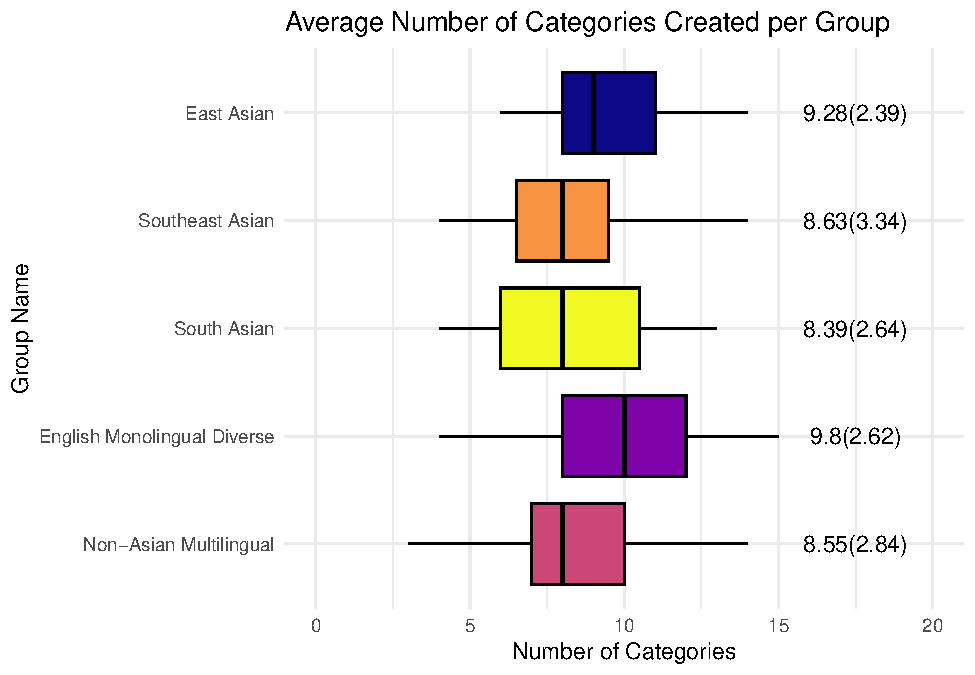
\includegraphics{DE3_papaja_files/figure-latex/unnamed-chunk-4-1.pdf}

\subsection{Error Patterns}\label{error-patterns}

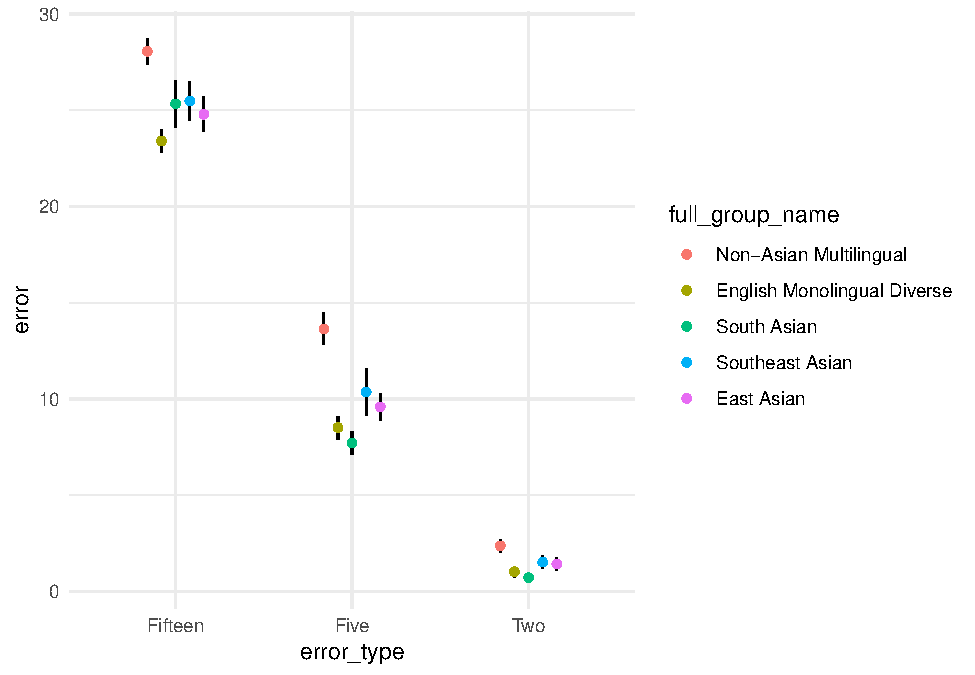
\includegraphics{DE3_papaja_files/figure-latex/unnamed-chunk-6-1.pdf}

\section{Discussion}\label{discussion}

\newpage

\section{References}\label{references}

\phantomsection\label{refs}
\begin{CSLReferences}{1}{0}
\bibitem[\citeproctext]{ref-R-papaja}
Aust, F., \& Barth, M. (2024). \emph{{papaja}: {Prepare} reproducible {APA} journal articles with {R Markdown}}. \url{https://doi.org/10.32614/CRAN.package.papaja}

\bibitem[\citeproctext]{ref-R-tinylabels}
Barth, M. (2023). \emph{{tinylabels}: Lightweight variable labels}. Retrieved from \url{https://cran.r-project.org/package=tinylabels}

\bibitem[\citeproctext]{ref-R-lubridate}
Grolemund, G., \& Wickham, H. (2011). Dates and times made easy with {lubridate}. \emph{Journal of Statistical Software}, \emph{40}(3), 1--25. Retrieved from \url{https://www.jstatsoft.org/v40/i03/}

\bibitem[\citeproctext]{ref-R-ggdist}
Kay, M. (2024). {ggdist}: Visualizations of distributions and uncertainty in the grammar of graphics. \emph{IEEE Transactions on Visualization and Computer Graphics}, \emph{30}(1), 414--424. \url{https://doi.org/10.1109/TVCG.2023.3327195}

\bibitem[\citeproctext]{ref-R-tibble}
Müller, K., \& Wickham, H. (2023). \emph{Tibble: Simple data frames}. Retrieved from \url{https://CRAN.R-project.org/package=tibble}

\bibitem[\citeproctext]{ref-R-base}
R Core Team. (2024). \emph{R: A language and environment for statistical computing}. Vienna, Austria: R Foundation for Statistical Computing. Retrieved from \url{https://www.R-project.org/}

\bibitem[\citeproctext]{ref-R-ggplot2}
Wickham, H. (2016). \emph{ggplot2: Elegant graphics for data analysis}. Springer-Verlag New York. Retrieved from \url{https://ggplot2.tidyverse.org}

\bibitem[\citeproctext]{ref-R-forcats}
Wickham, H. (2023a). \emph{Forcats: Tools for working with categorical variables (factors)}. Retrieved from \url{https://CRAN.R-project.org/package=forcats}

\bibitem[\citeproctext]{ref-R-stringr}
Wickham, H. (2023b). \emph{Stringr: Simple, consistent wrappers for common string operations}. Retrieved from \url{https://CRAN.R-project.org/package=stringr}

\bibitem[\citeproctext]{ref-R-tidyverse}
Wickham, H., Averick, M., Bryan, J., Chang, W., McGowan, L. D., François, R., \ldots{} Yutani, H. (2019). Welcome to the {tidyverse}. \emph{Journal of Open Source Software}, \emph{4}(43), 1686. \url{https://doi.org/10.21105/joss.01686}

\bibitem[\citeproctext]{ref-R-dplyr}
Wickham, H., François, R., Henry, L., Müller, K., \& Vaughan, D. (2023). \emph{Dplyr: A grammar of data manipulation}. Retrieved from \url{https://CRAN.R-project.org/package=dplyr}

\bibitem[\citeproctext]{ref-R-purrr}
Wickham, H., \& Henry, L. (2023). \emph{Purrr: Functional programming tools}. Retrieved from \url{https://CRAN.R-project.org/package=purrr}

\bibitem[\citeproctext]{ref-R-readr}
Wickham, H., Hester, J., \& Bryan, J. (2024). \emph{Readr: Read rectangular text data}. Retrieved from \url{https://CRAN.R-project.org/package=readr}

\bibitem[\citeproctext]{ref-R-tidyr}
Wickham, H., Vaughan, D., \& Girlich, M. (2024). \emph{Tidyr: Tidy messy data}. Retrieved from \url{https://CRAN.R-project.org/package=tidyr}

\end{CSLReferences}


\end{document}
